\section{Example of a SNAIL coupler}
\label{sec:snail}
\begin{figure}[H]
    \centering
    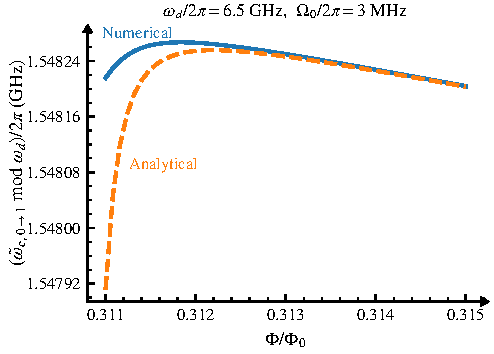
\includegraphics[width=0.9\linewidth]{chapter7/figures/SNAILss.pdf}
    \caption{Drive-induced sweet spot in a SNAIL--cavity system. Under continuous drive, the cavity transition energy exhibits a maximum near \(\Phi \simeq 0.311\,\Phi_0\), indicating reduced first-order flux susceptibility. Solid lines show numerical results and dashed lines show the perturbative prediction from Eq.~\eqref{perturbation energy}.}
    \label{fig:snail_ss}
\end{figure}

The superconducting nonlinear asymmetric inductive element (SNAIL) is a three-wave-mixing circuit element widely used for parametric amplification and gate operations.
When coupled capacitively to a cavity, the system Hamiltonian can be written as
\begin{equation}
\begin{aligned}
H =\;& \omega_s s^\dagger s 
+ \sum_j g_j (s + s^\dagger)^j
+ \omega_c c^\dagger c \\
&+ g (s + s^\dagger)(c + c^\dagger)
+ 2\Omega_0 \cos(\omega_d t) (s + s^\dagger).
\end{aligned}
\end{equation}
Here \(\omega_s\) is the SNAIL mode frequency, \(g_j\) are the nonlinear coefficients, \(g\) is the SNAIL--cavity coupling strength, \(s\) (\(c\)) is the SNAIL (cavity) mode operator, and \(\omega_d\) is the drive frequency.
The parameters \(\omega_s\), \(g_j\), \(g\), and \(\Omega_0\) are flux dependent through \(\Phi\).

To illustrate the generality of the drive-induced cancellation mechanism, the SNAIL is biased at \(\Phi = 0.3\,\Phi_0\), where the cubic nonlinearity \(g_3\) enables three-wave mixing.
At this operating point, \(g_3/2\pi \approx 67~\mathrm{MHz}\), \(\omega_s/2\pi = 6.59~\mathrm{GHz}\), and \(\omega_c/2\pi = 5~\mathrm{GHz}\).

A coherent drive with amplitude \(\Omega_0 = 3~\mathrm{MHz}\) at \(\omega_d = 6.5~\mathrm{GHz}\) produces a flux sweet spot in the cavity spectrum.
As shown in Fig.~\ref{fig:snail_ss}, the cavity transition energy, extracted using the procedure in App.~\ref{app:numerics}, develops a local maximum near \(\Phi \simeq 0.311\,\Phi_0\), consistent with vanishing first-order flux susceptibility.
The perturbative expression in Eq.~\eqref{perturbation energy} reproduces this sweet spot quantitatively, demonstrating that the drive-induced cancellation mechanism extends beyond the FTT to more general nonlinear, flux-dependent modes.